%% sample template file for a MSc Thesis
%% The default is with two sided setup:
\documentclass[%
oneside,    %% uncomment for onesided layout
project,    %% uncomment not thesis but project report
nosummary   %% uncomment if no summary page should be generated
]{USN-MSc}

% The following command removes the chapter names form the header
% (comment/remove) if you prefer to have them:
\pagestyle{plain}

% --- Bibliography setup ---
%%% default is the "ieee" style
\usepackage[style=ieee, sorting=none]{biblatex}
%%% If you want to use "author-year" style
%%% where `\cite{Foo2011}` generates "Foo et al. (2011)"
%%% and   `\parencite{Foo2011}` generates "(Foo et al. 2011)"
%%% then comment the line above and use
%\usepackage[style=authoryear]{biblatex}
%%% or
%%% if you want to use "alphabetic" style then use
%%% where `cite[Foo2011]` generates "[Foo11]"
%%% then comment the line above and use
%\usepackage[style=alphabetic]{biblatex}
%%% instead.
%% load the bib file:
\addbibresource{MScThesis.bib}

\usepackage{lipsum} % just for providing fill text used in this template
\usepackage{array} % for adjusting tables?
\usepackage{pdflscape} % for landscape pages

%These two are used to add frames to figures.
\usepackage{graphicx}
\usepackage[export]{adjustbox}

% --- general setup ---
%% Please fill in the following parameters:
\newcommand{\mytitle}{%
%% title:
Assignments for section 4 (W4.1-W4.5)
}

\newcommand{\mysubtitle}{%
%% master programme (for thesis only)
%% uncomment the appropriate one:
%%Electrical Power Engineering
%Energy and Environmental Technology
%Industrial IT and Automation
%Process Technology
}

\newcommand{\mykeywords}{%
%% keywords (for thesis only):
<keyword one, keyword two, \ldots>
}

\newcommand{\myauthor}{%
%% author(thesis) or group code (project):
223786 Lars Rikard Rådstoga
}

\newcommand{\myparticipants}{
%% group participants (for project only)
<First participant>\\
<Second participant>\\
<Third participant>\\
<Fourth participant>
}

\newcommand{\supervisor}{%
%% supervisor:
<Supervisor's Name>}

\begin{document}

% --- title page setup ---
%\USNtitlepage%
%%% Please provide the following information:
%%% #1 optional figure (set to {} if not wanted)
%{%
%  {\normalsize}
%  \begin{figure}[!ht]
%    \centering
%   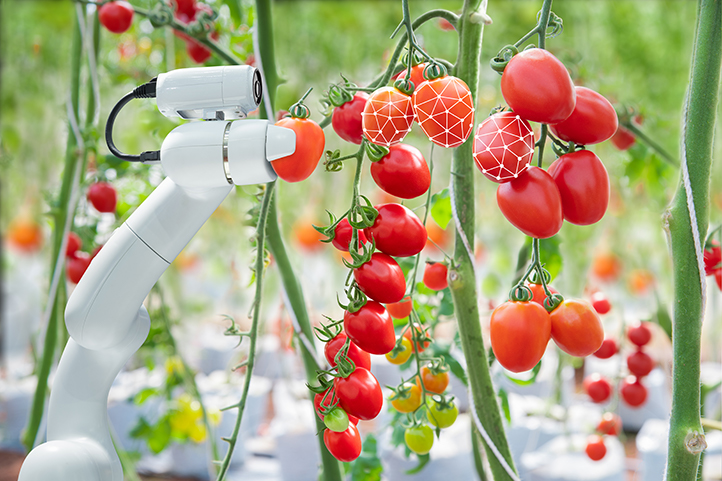
\includegraphics[width=0.8\textwidth]{TomatoPickerBot}
%   \label{fig:tomatoBot}
% \end{figure}
%}
% --- title page setup ---
\USNtitlepage%
%% Please provide the following information:
%% #1 optional figure (set to {} if not wanted)
{%
  {\normalsize}
   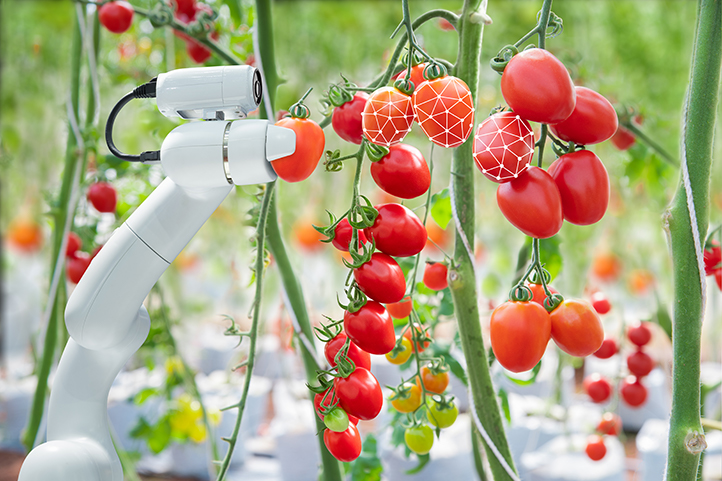
\includegraphics[width=\textwidth]{TomatoPickerBot}}
%% #2 Project partner:
{<Project partner>}
%% #3 Summary:
{%
\lipsum[6-7]
}


%\chapter*{Preface}
%\label{ch:preface}
%\addcontentsline{toc}{chapter}{Preface}
%\lipsum[1-3]
%\bigskip
%Porsgrunn, \today

%\myauthor %% for thesis
%\myparticipants %% for project


%% table of contents
\tableofcontents
\addcontentsline{toc}{chapter}{\contentsname}

%\listoffigures % out-comment if unwanted
%\addcontentsline{toc}{section}{\listfigurename}

%\listoftables  % out-comment if unwanted
%\addcontentsline{toc}{section}{\listtablename}


\chapter{Capabilities}
\label{ch:cap}
This chapter contains a reflection of the capabilities of an autonomous system.
\section{Reflection}
To better understand the required capabilities of an autonomous system it is sensible to reflect upon the degree of automation required with respect to the four sliders of autonomy \cite{murphy2000introduction}, see figure \ref{fig:fourSliders}.

\begin{figure}[!ht]
  \centering
  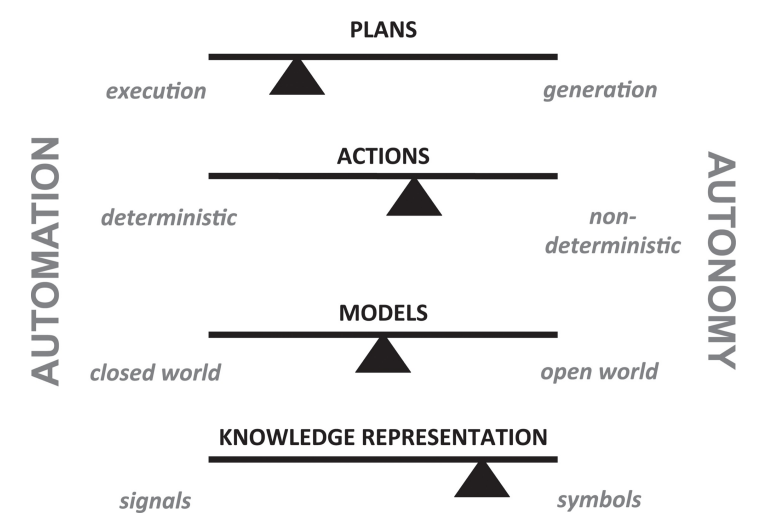
\includegraphics[width=0.80\textwidth, frame]{FourSlidersOfAutonomy}
  \caption{The four sliders of autonomy, an aid used to describe the degree of autonomy required for a system \cite{murphy2000introduction}.}
  \label{fig:fourSliders}
\end{figure}

The four sliders impact the degree of complexity of the system. 
A higher degree of autonomy implies on-the-go planning, this means that a system could be able to adapt and prioritize tasks in order to minimize cost functions. It can perform big-picture planning by actively doing tasks such as coordinating with other actors, considering refueling timing, and more to minimize usage costs.

Autonomous systems' actions adapt to wear and tear or change in environment by using noisy sensors and closed-loop control algorithms. The more open and the less static the world is, more features need to take action like this. Some applications such as assembly in a factory will be operable with few or no sensory feedback, but robots like the Mars Rover will need a lot so it can operate cautiously. 

The world model also impacts the degree of autonomy. In closed world examples, predictable environments such as a part of a factory, most of the world will be known a priori. In open world scenarios, however, the ground might be uneven or dirt can shift around. Objectives won't always appear in the same spots, etc. Open world models include less a priori information and more will be discovered a posteriori.

How knowledge is represented in the system is the last autonomy slider. In automated systems knowledge is mostly represented as signals such as GPS signals, sensory data and respective setpoints. E.g., to move from point A to B the automated robot would follow a coordinate-signal objective, but the autonomous robot would follow an order to move to fruit tree. This abstraction requires extra complexity.

\chapter{Frameworks}
\label{ch:frame}
This chapter contains a discussion on robotic frameworks.
\section{Discussion}

There are numerous frameworks and middleware options for robotics. Some options of which are dead projects, e.g. the Microsoft Robotics Studio, some are popular like the ROS framework, Gazebo, Rviz and Nvidia Isaac, and some might be under the radar like Hop. But the question is, do tools like these have what it takes to create intelligent AI based autonomous robots.

\begin{figure}[!ht]
  \centering
  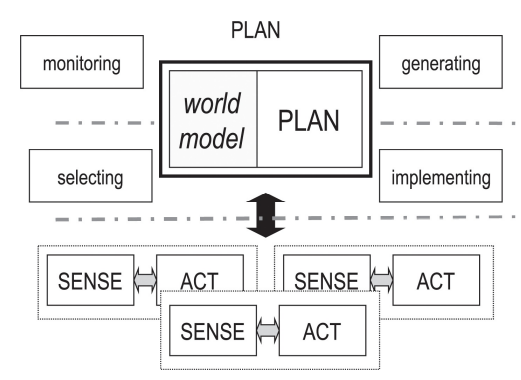
\includegraphics[width=0.80\textwidth, frame]{ReactiveAndDeliberativeLayers}
  \caption{The main functions within reactive and deliberative layers.}
  \label{fig:ReactDelib}
\end{figure}

As seen in figure \ref{fig:ReactDelib} an autonomous system can consist of multiple functions, these are often low coupled modules that require frameworks and/or middleware to work together. Such as ROS, the Robotic Operating System built upon Linux. Most importantly ROS includes infrastructure for communication between functions, this means that the ACT module can read information from the SENSE module in the reactive layer. ROS also comes with middleware that makes a lot of sensors and actuators work with minimal manual setup. Reactive layer functionality can then be created by fast-tracking sensory data to the ACT module where safety measures can be implemented, such as stop if unexpected obstacles appear. Deliberative layer functionality can then work asynchronously from the reactive. The deliberative layer can also subscribe to the sensory data and convert it to symbols that make up the world model. The four deliberative functions: generating, selecting, implementing, and monitoring can then able to work together to make intelligent decisions for the robot to achieve its goals.

\chapter{Industrial applications}
\label{ch:induApp}
This chapter contains a discussion regarding if and how autonomous systems can be used in industrial settings.
\section{Discussion}
Industrial plants today are already automated to a high degree and require operators to make reactive and preemptive measures to combat anomalies or unstable control. Automated systems take simple process inputs and regulating the process by minimizing the error to setpoints using algorithms such as PID to control actuators. This translates to the traditional sense, analyze, and act scheme depicted in gray in figure \ref{fig:Fig1Article1}. Instead, autonomous systems need to make more informed decisions, probably requiring data from multiple sources and the ability to make accurate predictions about future relevant developments in the relevant system.

\begin{figure}[!ht]
  \centering
  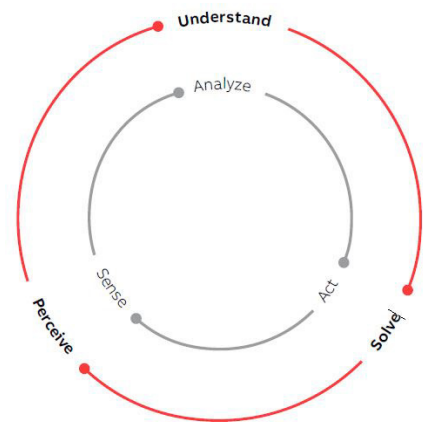
\includegraphics[width=0.50\textwidth, frame]{Fig1Article1}
  \caption{Loops in classical control systems (gray) and autonomous systems (red) \cite{GAMER2019454}}
  \label{fig:Fig1Article1}
\end{figure}

The scale between automation and autonomy is defined in different ways according to the field of study. Whether it is possible to implement autonomy to industrial settings depend on the definition of said scale. A definition of encapsulating categories of industrial systems can be seen in \ref{fig:Fig1Article2}. The automated system contains systematic process execution which can be as simple as hard coded arrays of coordinates and paths for a robot arm to follow. An intelligent automation system would in addition use sensory data to adapt to obstacles in the robot arms path, redirecting it. To truly reach autonomy the arm should also have self-governance and self-containedness. Self-governance meaning it should be able to do several high-level tasks like cooperating and decision-making without external help. Self-containedness is another branch of high-level tasks such as self-explanation and holistic affiliation, see figure \ref{fig:Tab3Article2} for explanations of some of these words. 

\begin{figure}[!ht]
  \centering
  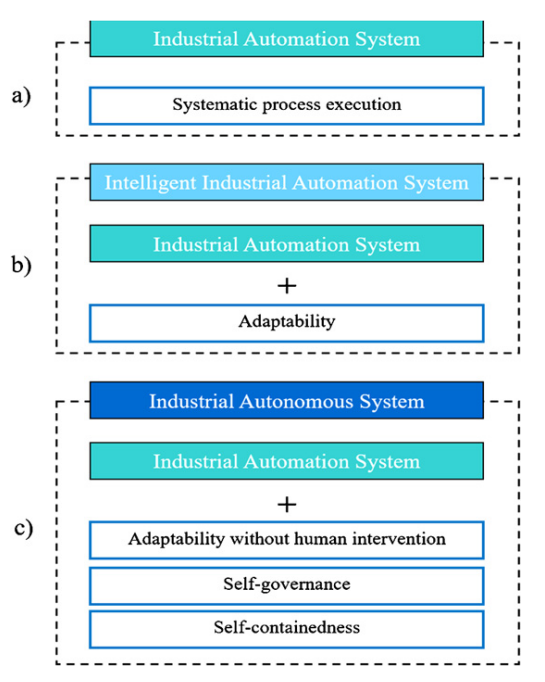
\includegraphics[width=0.50\textwidth, frame]{Figure1Article2}
  \caption{Differences between (classic) industrial automation systems, intelligent industrial automation systems, and industrial autonomous systems \cite{Müller}.}
  \label{fig:Fig1Article2}
\end{figure}


\begin{figure}[!ht]
  \centering
  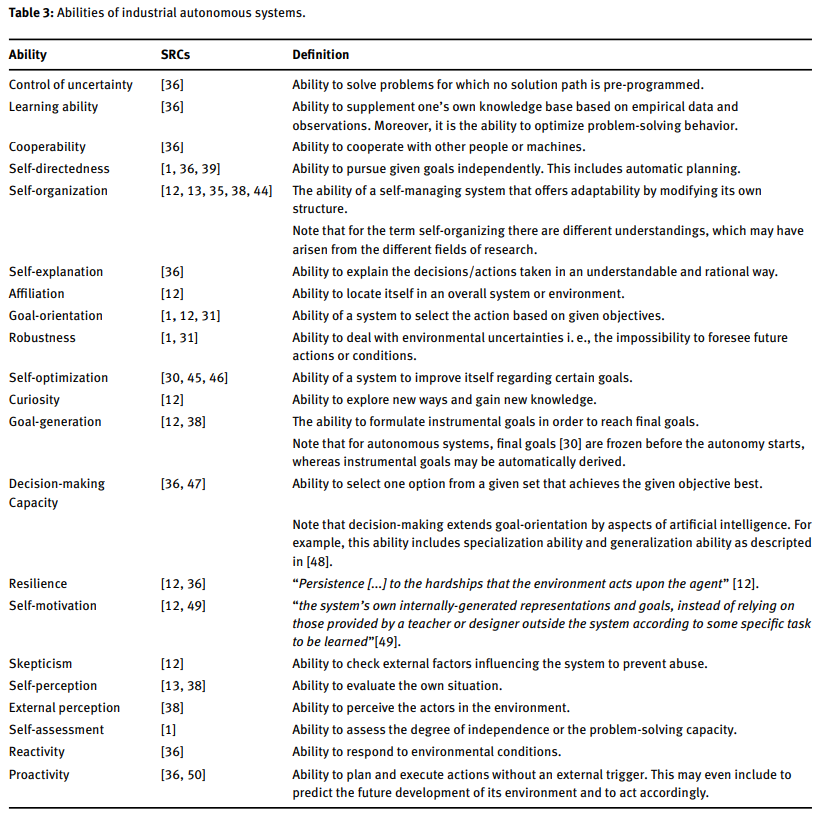
\includegraphics[width=0.90\textwidth, frame]{Table3Article2}
  \caption{Abilities of Industrial autonomous systems \cite{Müller}.}
  \label{fig:Tab3Article2}
\end{figure}



\chapter{Operational boundaries}
\label{ch:opBounds}
This chapter contains a definition of operational boundaries for the fruit-picker system.
\section{Definition}

Operational boundaries or operational design domain (ODD) is a definition of a systems operational area and constraints \cite{norwegiandefinitions}. This concerns the environment, equipment, and operations. 
Dynamic navigation task (DNT) is a set of tactical operations supported to operate in the ODD.
DNT Fallback is the predefined emergency procedure when ODD is exceeded.

\begin{figure}[!ht]
  \centering
  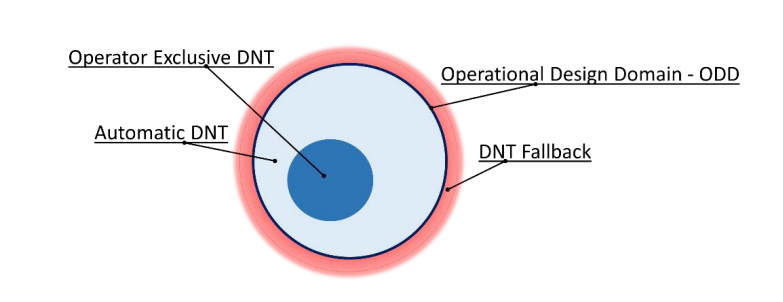
\includegraphics[width=0.80\textwidth, frame]{OperationalBoundsExample}
  \caption{Illustration of relationships between ODD, DNT and DNT Fallback \cite{norwegiandefinitions}.}
  \label{fig:OpBoundsEx}
\end{figure}

\section{Operator exclusive control}


\chapter{Overall capabilities of the fruit-picker system}
\label{ch:overalCap}
This chapter contains a description of all required capabilities: level of autonomy, main task description, HMI, and requirements for the robotic framework.
\section{Description}

% A dummy command that causes all bibliographyentries to be displayed
% even though there were not cited in the document. Used for demonstration
% purposes only in this template file.
~\nocite{*}

\cleardoublepage

% The bibliography should be displayed here...
%\printbibliography[heading=bibintoc]
% You rather like to call the bibliography "References"? Then use this instead:
\printbibliography[heading=bibintoc, title={References}]


%\appendix
%\renewcommand{\appendixname}{Paper} %% So we get 'Paper X' displayed instead


%\chapter[Short Title of Paper A]{Title of Paper A (probably very long and therefore not good to have in the header)}
%\label{paper-a}
%
%\paragraph{Note}
%Since some papers tend to have a rather long title it is good to provide the optional short title which then will be displayed in the table of contents and header instead of the long original title.
%On the openening page of the chapter the orginal \emph{long} title will be displayed.\bigskip
%
%\emph{Short descriptive text of paper follows here.}\bigskip
%
%The paper itself needs to be included in the published form as PDF on the next pages.
%This can be done using the \texttt{pdfpages} package by adding the command:
%
%\begin{verbatim}
%\includepdf{pages=-,openright}{Filename}
%\end{verbatim}
%
%You can omit the \texttt{.pdf} when specifying the \texttt{Filename}. Also you should include always include the option \texttt{openright} since it would look strange to have the paper starting at the back of the cover page.
%
%There are more options like only adding specific pages:
%\begin{verbatim}
%\includepdf{pages=2-6,openright}{Filename.pdf}
%\end{verbatim}

%For more options see Appendix~\ref{paper-b} where the most important pages of the \texttt{pdfpages} manual were inlcuded using \texttt{pdfpages}.


%%% Command to include a PDF file directly including all pages:


%\chapter[Short Title of Paper B]{Title of Paper B}
%\label{paper-b}
%Short descriptive text of paper follows here.
%
%Here we included the first five pages of the \texttt{pdfpages} manual itself.
%
%\includepdf[pages=1-5,openright]{fig/pdfpages}
%
\end{document}

%%% Local Variables:
%%% mode: latex
%%% TeX-master: t
%%% End:
